% Shared by every deck of the challenge (the presentation, and each level).
% Style: ../template/dcptalk.sty; this file and links.tex are found through
% TEXINPUTS (see deck.mk). Trimmed from the 2026 hylos decks' preamble.
\usepackage[fonts = paper, codedir = gen]{dcptalk}
\input{gen/pygments}
\graphicspath{{../common/images/}{../template/images/}}

\colorlet{accent}{blue!60!black}
\colorlet{accent2}{orange!80!black}
\colorlet{bad}{dcpbad}
\colorlet{good}{dcpgood}

% Links (\url, \href) in the accent colour, so they stand out
\hypersetup{colorlinks = true, urlcolor = accent, linkcolor = black}
\usetikzlibrary{shadows}

% ---------------------------------------------------------------- algebra
\newcommand\sel[1]{\sigma_{#1}}      % selection
\newcommand\proj[1]{\pi_{#1}}        % projection
\newcommand\ren[2]{\rho_{#1\to#2}}   % renaming
\newcommand\join{\bowtie}            % natural join
\newcommand\att[1]{\mathit{#1}}      % an attribute
\newcommand\val[1]{\mathrm{#1}}      % a value
\newcommand\rel[1]{\mathit{#1}}      % a relation (table) name

% ---------------------------------------------------------------- code
% Lean in blue (dcptalk's Rocq box), SQL in orange
\newtcolorbox{mainbox}[1][]{enhanced, drop fuzzy shadow southeast,
  boxrule = 0pt, colframe = orange!12, colback = orange!12,
  halign = flush left, #1}
\makeatletter
\NewDocumentCommand\leanblock{O{} m}{\dcp@code{bluebox}{#1}{#2}}
\NewDocumentCommand\mainblock{O{} m}{\dcp@code{mainbox}{#1}{#2}}
\makeatother
% Under a Lean block that has not been type-checked: statements only, with
% definitions left to the reader
\newcommand\sketch{\par{\hfill\footnotesize\textcolor{gray}{(sketch: the
  types are yours to design; your job is to replace each \code{sorry})}\par}}

% ---------------------------------------------------------------- tags
% A tag in the top-right corner: which level of the challenge a frame is
% about. At the end of the frame, like \slideref.
\NewDocumentCommand\worktag{O{accent} m}{%
  \begin{tikzpicture}[overlay, remember picture, alt = {Tag: #2}]
    \node[anchor = north east, draw = #1, fill = #1!12, text = #1,
      rounded corners = 2pt, font = \footnotesize\bfseries, inner sep = 3pt]
      at ($(current page.north east) + (-4mm, -4mm)$) {#2};
  \end{tikzpicture}\par}
\colorlet{levelcol}{black!70}
\newcommand\leveltag[1]{\worktag[levelcol]{Level #1}}
\newcommand\stretchtag{\worktag[levelcol]{Stretch}}
% Every frame of a level is either theory (on paper) or Lean (on the
% computer), and says so in its tag, in its own colour
\colorlet{theorycol}{orange!80!black}
\colorlet{leancol}{blue!60!black}
\newcommand\theorytag[1]{\worktag[theorycol]{Level #1 · Theory}}
\newcommand\leantag[1]{\worktag[leancol]{Level #1 · Lean}}
\newcommand\setuptag{\worktag[leancol]{Setup · Lean}}

% ---------------------------------------------------------------- levels
% Each level is its own PDF, at <challenge>/level-<id>/level-<id>.pdf;
% the presentation is <challenge>/slides.pdf. The links are absolute, so
% they work from a downloaded copy too.
\newcommand\challengeurl{https://dcastrop.github.io/tex/2026-papc-challenge}
% \levellink{2f}: "Level 2F", linked to its PDF
\newcommand\levellink[1]{%
  \href{\challengeurl/level-#1/level-#1.pdf}{Level \MakeUppercase{#1}}}
\newcommand\challengelink[1]{\href{\challengeurl/slides.pdf}{#1}}

% \leveltitle{2F}{title}{track}{after}{next}: a level's title page. No
% footer, not counted; the club, not a speaker; no date. The last line
% links the levels before and after, and the whole challenge.
\NewDocumentCommand\leveltitle{m m m m m}{%
  \stepcounter{dcpskipped}%
  \begin{frame}
    \thispagestyle{talknofooter}
    \vfill
    \begin{center}
      {\large\challengelink{We Have a Challenge for You!}\par}
      \medskip
      % Latin Modern's 17pt design has a tight word space at \Huge
      {\Huge\spaceskip = .36em\relax Level #1\par}
      \smallskip
      {\Large #2\par}
      \smallskip
      {\color{black!60}#3\par}
      \vspace{3mm}
      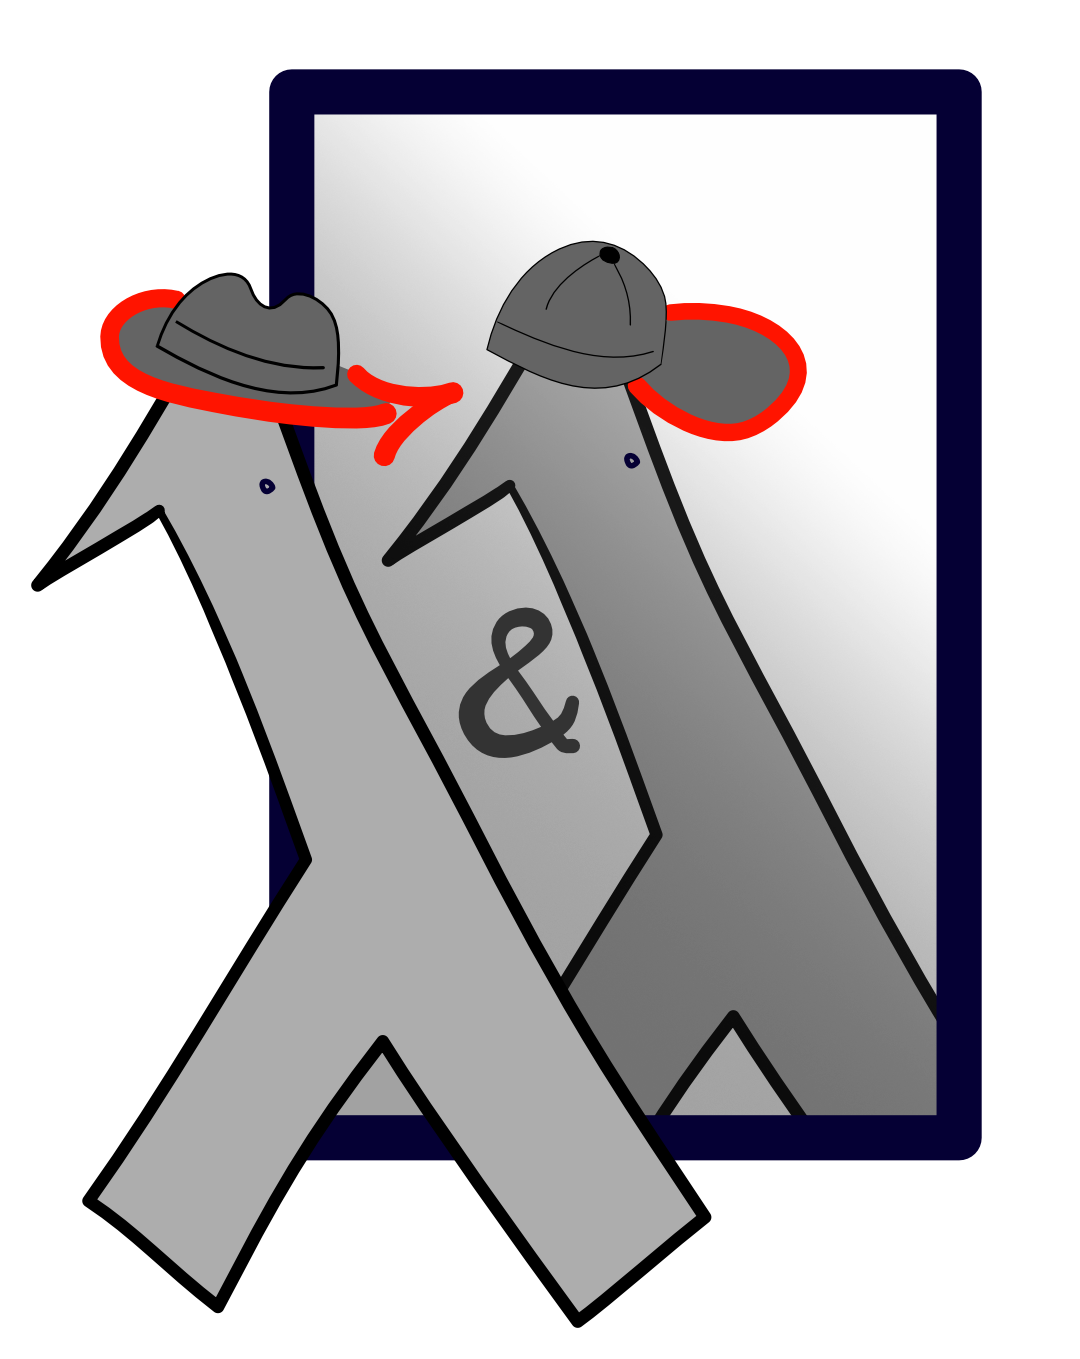
\includegraphics[height = 16mm, alt = {The Proofs and Programs Club
        logo: a lambda in a hat and its reflection in a mirror, wearing a
        different hat, with an ampersand between them}]{papc-logo.png}\par
      \smallskip
      The Proofs and Programs Club @ RHUL\par
      {\small\url{https://papc-rhul.github.io/}\par}
      \vspace{3mm}
      {\small #4\quad·\quad #5\quad·\quad\challengelink{All the
        levels}\par}
    \end{center}
    \vfill
    \begin{tikzpicture}[overlay, remember picture]
      \node[anchor = south east, inner sep = 0pt]
        at ($(current page.south east) + (-4mm, 4mm)$)
        {
\includegraphics[height = 8mm, alt = {Royal Holloway, University
          of London logo}]{RHULLogo.png}};
    \end{tikzpicture}
  \end{frame}}

% Inside a level, a part frame opens the theory and another the Lean
\newcommand\theorypart[1]{\partframe{Theory, on Paper}{#1}}
\newcommand\leanpart[1]{\partframe{Lean, on Your Computer}{#1}}

% \defn{Definition 1.1 (Table)}{text}: a definition, law or fact, in a
% box with a theory-coloured rule on its left
\NewDocumentCommand\defn{m +m}{%
  \begin{tcolorbox}[enhanced, boxrule = 0pt, colback = white,
      colframe = white, borderline west = {2.5pt}{0pt}{theorycol},
      left = 3mm, right = 2mm, top = 1mm, bottom = 1mm,
      halign = flush left, drop fuzzy shadow southeast]
    \textbf{#1}\enspace #2
  \end{tcolorbox}}
% The end of a proof
\newcommand\proofend{\hfill\rule{1ex}{1ex}}
% Booleans, true, false, natural numbers
\newcommand\B{\mathbb{B}}
\newcommand\true{\mathsf{true}}
\newcommand\false{\mathsf{false}}
\newcommand\N{\mathbb{N}}

% ---------------------------------------------------------------- refs
% Inside \slideref: the next reference starts on a new line
\newcommand\rfsep{\\}
% References sit 4mm from the bottom, one per line, under a short rule.
% Their alt text drops the URLs of \href (\lnk), keeping the link text.
\makeatletter
\RenewDocumentCommand\slideref{+m}{%
  \let\dcp@href\href
  \let\href\@secondoftwo
  \protected@edef\dcp@refalt{#1}%
  \let\href\dcp@href
  \begin{tikzpicture}[overlay, remember picture,
      alt = {References: \dcp@refalt}]
    \node[anchor = south west, font = \tiny, text width = 150mm,
      align = left] at ($(current page.south west) + (10mm, 4mm)$)
      {\textcolor{black!40}{\rule{25mm}{0.4pt}}\\[0.3ex] #1};
  \end{tikzpicture}\par}
\makeatother

% Book sections: \deflink{key}{book and number}{title}{url} in links.tex
% (read with # and _ as ordinary characters, for the URLs); \lnk{key}
% prints "FPIL 7.3 Title", the title linked.
\newcommand\deflink[4]{%
  \if\relax\detokenize{#2}\relax
    \expandafter\gdef\csname dcplink@#1\endcsname{\href{#4}{\textbf{#3}}}%
  \else
    \expandafter\gdef\csname dcplink@#1\endcsname{#2 \href{#4}{\textbf{#3}}}%
  \fi}
\newcommand\lnk[1]{%
  \ifcsname dcplink@#1\endcsname \csname dcplink@#1\endcsname
  \else \errmessage{Unknown link #1}\fi}
\begingroup
  \catcode`\#=12 \catcode`\_=12
  \deflink{fpil}{}{Functional Programming in Lean (FPIL)}{https://lean-lang.org/functional_programming_in_lean/}
\deflink{tpil}{}{Theorem Proving in Lean 4 (TPIL)}{https://lean-lang.org/theorem_proving_in_lean4/}
\deflink{mil}{}{Mathematics in Lean (MIL)}{https://leanprover-community.github.io/mathematics_in_lean/}
\deflink{mathlib}{}{Mathlib documentation}{https://leanprover-community.github.io/mathlib4_docs/}
\deflink{loogle}{}{Loogle}{https://loogle.lean-lang.org/}
\deflink{games}{}{Lean Game Server}{https://adam.math.hhu.de/}
\deflink{fpil-eval}{FPIL 1.1}{Evaluating Expressions}{https://lean-lang.org/functional_programming_in_lean/Getting-to-Know-Lean/Evaluating-Expressions/#evaluating}
\deflink{fpil-struct}{FPIL 1.4}{Structures}{https://lean-lang.org/functional_programming_in_lean/Getting-to-Know-Lean/Structures/#structures}
\deflink{fpil-data}{FPIL 1.5}{Datatypes and Patterns}{https://lean-lang.org/functional_programming_in_lean/Getting-to-Know-Lean/Datatypes-and-Patterns/#datatypes-and-patterns}
\deflink{fpil-poly}{FPIL 1.6}{Polymorphism}{https://lean-lang.org/functional_programming_in_lean/Getting-to-Know-Lean/Polymorphism/#polymorphism}
\deflink{fpil-props}{FPIL}{Interlude: Propositions, Proofs, and Indexing}{https://lean-lang.org/functional_programming_in_lean/Interlude___-Propositions___-Proofs___-and-Indexing/#props-proofs-indexing}
\deflink{fpil-arrays}{FPIL 3.4}{Arrays and Indexing}{https://lean-lang.org/functional_programming_in_lean/Overloading-and-Type-Classes/Arrays-and-Indexing/}
\deflink{fpil-eqord}{FPIL 3.5.3}{Equality and Ordering}{https://lean-lang.org/functional_programming_in_lean/Overloading-and-Type-Classes/Standard-Classes/#equality-and-ordering}
\deflink{fpil-hash}{FPIL 3.5.4}{Hashing}{https://lean-lang.org/functional_programming_in_lean/Overloading-and-Type-Classes/Standard-Classes/#hashing}
\deflink{fpil-deriving}{FPIL 3.5.5}{Deriving Standard Classes}{https://lean-lang.org/functional_programming_in_lean/Overloading-and-Type-Classes/Standard-Classes/#deriving-standard-classes}
\deflink{fpil-indexed}{FPIL 7.1}{Indexed Families}{https://lean-lang.org/functional_programming_in_lean/Programming-with-Dependent-Types/Indexed-Families/#indexed-families}
\deflink{fpil-universe}{FPIL 7.2}{The Universe Design Pattern}{https://lean-lang.org/functional_programming_in_lean/Programming-with-Dependent-Types/The-Universe-Design-Pattern/#universe-pattern}
\deflink{fpil-tq}{FPIL 7.3}{Worked Example: Typed Queries}{https://lean-lang.org/functional_programming_in_lean/Programming-with-Dependent-Types/Worked-Example___-Typed-Queries/#typed-queries}
\deflink{fpil-tqex}{FPIL 7.3.6}{Exercises (Typed Queries: Dates, Nullable Types, ...)}{https://lean-lang.org/functional_programming_in_lean/Programming-with-Dependent-Types/Worked-Example___-Typed-Queries/#typed-query-exercises}
\deflink{fpil-pitfalls}{FPIL 7.5}{Pitfalls of Programming with Dependent Types}{https://lean-lang.org/functional_programming_in_lean/Programming-with-Dependent-Types/Pitfalls-of-Programming-with-Dependent-Types/#dependent-type-pitfalls}
\deflink{fpil-tactics}{FPIL}{Interlude: Tactics, Induction, and Proofs}{https://lean-lang.org/functional_programming_in_lean/Interlude___-Tactics___-Induction___-and-Proofs/#tactics-induction-proofs}
\deflink{fpil-indother}{FPIL Interlude,}{Induction on Other Datatypes}{https://lean-lang.org/functional_programming_in_lean/Interlude___-Tactics___-Induction___-and-Proofs/#induction-other-types}
\deflink{fpil-tail}{FPIL 8.1}{Tail Recursion}{https://lean-lang.org/functional_programming_in_lean/Programming___-Proving___-and-Performance/Tail-Recursion/#tail-recursion}
\deflink{fpil-equiv}{FPIL 8.2}{Proving Equivalence}{https://lean-lang.org/functional_programming_in_lean/Programming___-Proving___-and-Performance/Proving-Equivalence/#proving-tail-rec-equiv}
\deflink{fpil-arrterm}{FPIL 8.3}{Arrays and Termination}{https://lean-lang.org/functional_programming_in_lean/Programming___-Proving___-and-Performance/Arrays-and-Termination/#array-termination}
\deflink{fpil-fin}{FPIL 8.5}{Bounded Numbers}{https://lean-lang.org/functional_programming_in_lean/Programming___-Proving___-and-Performance/Bounded-Numbers/#Fin}
\deflink{fpil-insort}{FPIL 8.6}{Insertion Sort and Array Mutation}{https://lean-lang.org/functional_programming_in_lean/Programming___-Proving___-and-Performance/Insertion-Sort-and-Array-Mutation/#insertion-sort-mutation}
\deflink{tpil-pat}{TPIL 3.1}{Propositions as Types}{https://lean-lang.org/theorem_proving_in_lean4/Propositions-and-Proofs/#propositions-as-types}
\deflink{tpil-forall}{TPIL 4.1}{The Universal Quantifier}{https://lean-lang.org/theorem_proving_in_lean4/Quantifiers-and-Equality/#the-universal-quantifier}
\deflink{tpil-eq}{TPIL 4.2}{Equality}{https://lean-lang.org/theorem_proving_in_lean4/Quantifiers-and-Equality/#equality}
\deflink{tpil-calc}{TPIL 4.3}{Calculational Proofs}{https://lean-lang.org/theorem_proving_in_lean4/Quantifiers-and-Equality/#calculational-proofs}
\deflink{tpil-basic}{TPIL 5.2}{Basic Tactics}{https://lean-lang.org/theorem_proving_in_lean4/Tactics/#basic-tactics}
\deflink{tpil-rw}{TPIL 5.6}{Rewriting}{https://lean-lang.org/theorem_proving_in_lean4/Tactics/#rewriting}
\deflink{tpil-simp}{TPIL 5.7}{Using the Simplifier}{https://lean-lang.org/theorem_proving_in_lean4/Tactics/#using-the-simplifier}
\deflink{tpil-ctors}{TPIL 7.2}{Constructors with Arguments}{https://lean-lang.org/theorem_proving_in_lean4/Inductive-Types/#constructors-with-arguments}
\deflink{tpil-recdata}{TPIL 7.5}{Other Recursive Data Types}{https://lean-lang.org/theorem_proving_in_lean4/Inductive-Types/#other-recursive-data-types}
\deflink{tpil-indtac}{TPIL 7.6}{Tactics for Inductive Types}{https://lean-lang.org/theorem_proving_in_lean4/Inductive-Types/#tactics-for-inductive-types}
\deflink{tpil-families}{TPIL 7.7}{Inductive Families}{https://lean-lang.org/theorem_proving_in_lean4/Inductive-Types/#inductive-families}
\deflink{tpil-match}{TPIL 8.1}{Pattern Matching}{https://lean-lang.org/theorem_proving_in_lean4/Induction-and-Recursion/#pattern-matching}
\deflink{tpil-structrec}{TPIL 8.3}{Structural Recursion and Induction}{https://lean-lang.org/theorem_proving_in_lean4/Induction-and-Recursion/#structural-recursion-and-induction}
\deflink{tpil-wf}{TPIL 8.5}{Well-Founded Recursion and Induction}{https://lean-lang.org/theorem_proving_in_lean4/Induction-and-Recursion/#well-founded-recursion-and-induction}
\deflink{tpil-funind}{TPIL 8.6}{Functional Induction}{https://lean-lang.org/theorem_proving_in_lean4/Induction-and-Recursion/#functional-induction}
\deflink{tpil-dec}{TPIL 10.8}{Decidable Propositions}{https://lean-lang.org/theorem_proving_in_lean4/Type-Classes/#decidable-propositions}
\deflink{mil-sets}{MIL 4.1}{Sets}{https://leanprover-community.github.io/mathematics_in_lean/C04_Sets_and_Functions.html#sets}
\deflink{mil-finset}{MIL 6.1}{Finsets and Fintypes}{https://leanprover-community.github.io/mathematics_in_lean/C06_Discrete_Mathematics.html#finsets-and-fintypes}
\deflink{ml-finset}{Mathlib docs,}{Mathlib.Data.Finset.Defs}{https://leanprover-community.github.io/mathlib4_docs/Mathlib/Data/Finset/Defs.html}
\deflink{ml-multiset}{Mathlib docs,}{Mathlib.Data.Multiset.Defs}{https://leanprover-community.github.io/mathlib4_docs/Mathlib/Data/Multiset/Defs.html}
\deflink{ahv}{S. Abiteboul, R. Hull, V. Vianu.}{Foundations of Databases}{https://webdam.di.ens.fr/Alice/}
\deflink{ahv3}{Abiteboul, Hull, Vianu, Foundations of Databases (1995), ch. 3:}{The Relational Model}{https://webdam.di.ens.fr/Alice/pdfs/Chapter-3.pdf}
\deflink{ahv4}{Abiteboul, Hull, Vianu, Foundations of Databases (1995), ch. 4:}{Conjunctive Queries}{https://webdam.di.ens.fr/Alice/pdfs/Chapter-4.pdf}
\deflink{ahv5}{Abiteboul, Hull, Vianu, Foundations of Databases (1995), ch. 5:}{Adding Negation: Algebra and Calculus}{https://webdam.di.ens.fr/Alice/pdfs/Chapter-5.pdf}
\deflink{ahv6}{Abiteboul, Hull, Vianu, Foundations of Databases (1995), ch. 6:}{Static Analysis and Optimization}{https://webdam.di.ens.fr/Alice/pdfs/Chapter-6.pdf}
\deflink{nng}{}{Natural Number Game}{https://adam.math.hhu.de/}
\deflink{tpil-stt}{TPIL 2.1}{Simple Type Theory}{https://lean-lang.org/theorem_proving_in_lean4/Dependent-Type-Theory/#simple-type-theory}
\deflink{tpil-fun}{TPIL 2.3}{Function Abstraction and Evaluation}{https://lean-lang.org/theorem_proving_in_lean4/Dependent-Type-Theory/#function-abstraction-and-evaluation}
\deflink{tpil-defs}{TPIL 2.4}{Definitions}{https://lean-lang.org/theorem_proving_in_lean4/Dependent-Type-Theory/#definitions}
\deflink{tpil-split}{TPIL 5.8}{Split Tactic}{https://lean-lang.org/theorem_proving_in_lean4/Tactics/#split-tactic}
\deflink{fpil-types}{FPIL 1.2}{Types}{https://lean-lang.org/functional_programming_in_lean/Getting-to-Know-Lean/Types/#getting-to-know-types}
\deflink{fpil-fun}{FPIL 1.3}{Functions and Definitions}{https://lean-lang.org/functional_programming_in_lean/Getting-to-Know-Lean/Functions-and-Definitions/#functions-and-definitions}
\deflink{fpil-classes}{FPIL 3.2}{Type Classes and Polymorphism}{https://lean-lang.org/functional_programming_in_lean/Overloading-and-Type-Classes/Type-Classes-and-Polymorphism/#tc-polymorphism}
\deflink{tpil-proplogic}{TPIL 3.3}{Propositional Logic}{https://lean-lang.org/theorem_proving_in_lean4/Propositions-and-Proofs/#propositional-logic}
\deflink{tpil-classical}{TPIL 3.5}{Classical Logic}{https://lean-lang.org/theorem_proving_in_lean4/Propositions-and-Proofs/#classical-logic}
\deflink{tpil-exists}{TPIL 4.4}{The Existential Quantifier}{https://lean-lang.org/theorem_proving_in_lean4/Quantifiers-and-Equality/#the-existential-quantifier}

\endgroup

% ---------------------------------------------------------------- tables
% A table whose first row is its header, for the tagged PDF
\newcommand\headerrow{\tagpdfsetup{table/header-rows = {1}}}

% A small named table: \smalltable{name}{column spec}{header & ...}{rows}
\NewDocumentCommand\smalltable{m m m +m}{%
  \begin{tabular}[t]{@{}c@{}}
    #1\\[2pt]
    {\headerrow\begin{tabular}{#2}
      \hline #3 \\ \hline #4 \\ \hline
    \end{tabular}}
  \end{tabular}}

% ---------------------------------------------------------------- Lean
% \rds{key1, key2}: book sections (links.tex keys), one per line
\ExplSyntaxOn
\NewDocumentCommand \rds { m }
  {
    \seq_set_from_clist:Nn \l_tmpa_seq {#1}
    \seq_set_map:NNn \l_tmpb_seq \l_tmpa_seq { \lnk {##1} }
    \seq_use:Nn \l_tmpb_seq { \newline }
  }
\ExplSyntaxOff

% \ex{2.1}: the number of an exercise, in bold
\newcommand\ex[1]{\textbf{#1}\enspace}

% \levelframe{level}{title}{build}{prove}{rows}: the first frame of a
% level: what to build and prove, then a table of what to learn first, each
% row with the book sections to read (rows: "skill & \rds{keys} \\")
\NewDocumentCommand\levelframe{m m +m +m +m}{%
  \begin{frame}
    \frametitle{#2}
    \begin{sticky}
      \textbf{Build}: #3\par
      \textbf{Prove}: #4\par
    \end{sticky}
    \medskip
    {\centering\small\renewcommand\arraystretch{1.25}
      {\headerrow\begin{tabular}{@{}>{\raggedright\arraybackslash}p{68mm}@{\qquad}>{\raggedright\arraybackslash}p{78mm}@{}}
        \hline
        \textbf{First, learn to} & \textbf{Read} \\ \hline
        #5
        \hline
      \end{tabular}}\par}
    \leveltag{#1}
  \end{frame}}

% ---------------------------------------------------------------- footer
% "frame/total", bottom right. ltx-talk counts frames, not overlays.
\EditInstance{footer}{std}{
  color         = black!50,
  font          = \hfill\scriptsize,
  element-order = {framenumber, totalframes},
  separator     = /,
  right-hspace  = 4mm,
}

% Title frames have no footer, and are not counted
% (\stepcounter{dcpskipped} before them). A counter of our own: ltx-talk's
% frame counter also sets the PDF page labels.
\makeatletter
\newcounter{dcpskipped}
\def\ps@talknofooter{\ps@talk\def\@oddfoot{}\let\@evenfoot\@oddfoot}
% Part frames: no footer, not counted
\NewCommandCopy\dcp@partframe\partframe
\RenewDocumentCommand\partframe{m m}{\stepcounter{dcpskipped}%
  \dcp@partframe{#1}{#2\thispagestyle{talknofooter}}}
\ExplSyntaxOn
\property_new:nnnn { dcpskipped } { shipout } { 0 } { \int_use:N \c@dcpskipped }
\AddToHook { enddocument / afterlastpage }
  { \property_record:nn { dcp-lastpage } { dcpskipped } }
\cs_set:Npn \@framenumber { \int_eval:n { \c@frame - \c@dcpskipped } }
\cs_set:Npn \@totalframes
  {
    \int_eval:n
      {
          \property_ref:nn { lastpage } { frames }
        - \property_ref:nn { dcp-lastpage } { dcpskipped }
      }
  }
\ExplSyntaxOff
\makeatother
